\documentclass[11pt]{article}
\date{}
\renewcommand\abstractname{\fontsize{14pt}{0}\textbf{Abstract}\selectfont}

\usepackage[left=25mm, right=25mm, top=25mm, bottom=25mm, includehead=false, includefoot=false]{geometry}

\usepackage{graphicx}
\usepackage{url}
\usepackage[round,semicolon]{natbib}  % Citation styles https://www.sharelatex.com/learn/Natbib_citation_styles
\bibliographystyle{humannat}
\renewcommand{\bibsection}{}
\renewcommand{\bibhang}{\setlength{-1px}}


\usepackage{authblk} % For author lists
\renewcommand\Authfont{\fontsize{11}{1}\selectfont}
\renewcommand\Affilfont{\fontsize{9}{1}\selectfont}

\renewcommand*\footnoterule{}

\usepackage[table]{xcolor}
\usepackage[parfill]{parskip} % Line between paragraphs
\usepackage{amsmath}
\pagenumbering{arabic} 

\usepackage{sectsty}
\allsectionsfont{\sffamily}

\usepackage[pdftex]{hyperref} 
\hypersetup{pdfborder={0 0 0} }


% **************  TITLE AND AUTHOR INFORMATION **************

\title{\sffamily\fontsize{16}{0}\textbf{An agent-based model to investigate the effects of social segregation around the clock on social disparities in health attitudes and dietary behaviours.}}

\author[1]{Cl{\' e}mentine Cottineau}
\author[2]{Julien Perret}
\author[3,4]{Romain Reuillon}
\author[5]{S{\' e}bastien Rey-Coyrehourcq}
\author[3]{Julie Vall{\' e}e}
\affil[1]{Centre for Advanced Spatial Analysis, University College London, UK}
\affil[2]{COGIT, IGN, Paris, France}
\affil[3]{UMR 8504 G{\' e}ographie-cit{\' e}s, Paris, France}
\affil[4]{Institut des Syst{\` e}mes Complexes Paris Ile-de-France, France}
\affil[5]{UMR 6266 IDEES, Universit{\' e} de Rouen, France}

\begin{document}


\maketitle

% **************  ABSTRACT  **************

\begin{abstract}
\noindent
\setlength{\parindent}{0pt}
$ $ \\ {\bf Keywords:} 

\end{abstract}


% **************  MAIN BODY OF THE PAPER **************

\section{Introduction}

\subsection{The impact of the residential context and activity space on health behaviour of social groups}

\subsection{Agent-based modelling of spatial dietary practice}	

\subsection{Spatio-temporal segregation in the Paris region}	

\subsection{Social disparities of health behaviours}

\subsection{Neighbourhood effects on diet}

% ************** 

\section{Methods}

\subsection{Synthetique population generation}

\subsection{Individual data on dietary habits}

% ************** 

\section{Spatial Segregation of social behaviour: an agent-based model}

\subsection{Opinions and behaviour at initialisation}

\subsection {Changing behaviour}


\begin{figure}[htbp] \begin{center} 
\resizebox{0.9\textwidth}{!}{ 
	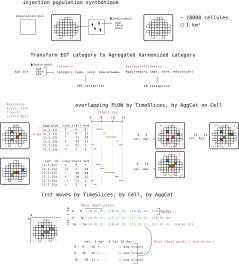
\includegraphics{schema_compute_EGT.png}
} \caption{Description of synthetic population generation} \label{fig:synthetic} \end{center} \end{figure} %



\begin{equation}
a^2 + b^2 = c^2
\tag*{Equation 1}
\end{equation}

\begin{figure}[htbp] 
\begin{center} 
\resizebox{0.9\textwidth}{!}{ 
	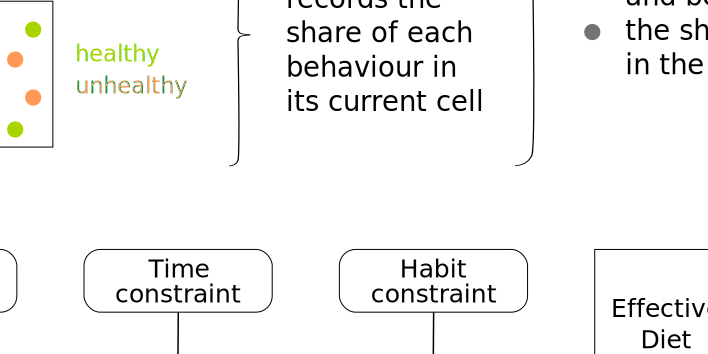
\includegraphics{desc_mechanisms_shem.png}
} \caption{Description of interaction, opinion and behaviour dynamics} 
\label{fig:mechanisms} 
\end{center} 
\end{figure} %


\begin{figure}[htbp] 
\begin{center} 
\resizebox{0.9\textwidth}{!}{ 
	\includegraphics{desc_mechanisms_switch_shem.png}
} \caption{Details of behaviour change} \label{fig:mechanisms_behaviour} 
\end{center} 
\end{figure} %


\subsection{Parameterization}


% ************** 

\section{Results}

% ************** 
\section{Discussion and Conclusion}



% \hfill \break
% \itshape{This is a sub, subheading}\normalfont

% \hfill\break

%
%
%\begin{table}[htp]
%
%\begin{center}
%\begin{tabular}{c c c c}
%\arrayrulecolor{black}
%\hline 
%This & Is & A & Table\\
%\arrayrulecolor{lightgray}
%\hline 
%\arrayrulecolor{black}
%Label & 0.1 & 0.2 & 0.3\\
%Label & 1.0 & 2.0 & 3.0\\
%\hline
%\end{tabular}
%\end{center}
%\label{first_table}
%\caption{This is a table caption}
%\end{table}%
%
%
%
%\begin{equation}
%a^2 + b^2 = c^2
%\tag*{Equation 1}
%\end{equation}


\section{References}


\bibliography{h24}


\end{document}
